\subsubsection{Requerimiento funcionales}

\begin{table}[!htb]
    \centering
    \caption{Plantilla de los requerimientos}
    \begin{tabular}{|p{3cm}|p{10cm}|}
    \hline
    \textbf{Identificador} & \textit{ID único que identifica el requisito funcional.} \\ \hline
    \textbf{Nombre} & \textit{Nombre descriptivo del requisito funcional.} \\ \hline
    \textbf{Rol} & \textit{Rol del usuario relacionado con este requisito.} \\ \hline
    \textbf{Funcionalidad} & \textit{Descripción detallada de la funcionalidad que se espera.} \\ \hline
    \textbf{Resultado} & \textit{Resultado esperado después de ejecutar la funcionalidad.} \\ \hline
    \textbf{Precondición} & \textit{Condiciones que deben cumplirse antes de ejecutar este requisito.} \\ \hline
    \textbf{Postcondición} & \textit{Estado esperado del sistema después de ejecutar el requisito.} \\ \hline
    \textbf{Flujo Normal de Eventos} & \textit{Secuencia típica de pasos para cumplir el requisito.} \\ \hline
    \textbf{Flujo Alternativo y Excepciones} & \textit{Descripciones de posibles desviaciones o errores en el flujo.} \\ \hline
    \end{tabular}
    \label{tabla:req-funcionales}
\end{table}
\FloatBarrier


\begin{table}[htb!]
    \centering
    \caption{Requisito Funcional RF-01}
\begin{tabular}{|p{4cm}|p{12cm}|}
\hline
\textbf{Campo} & \textbf{Descripcion} \\ \hline
\textbf{Identificador} & RF-01 \\ \hline
\textbf{Nombre} & Gestionar Roles \\ \hline
\textbf{Rol} & Administrador \\ \hline
\textbf{Funcionalidad} & Crear, editar y eliminar roles en el sistema. \\ \hline
\textbf{Resultado} & Permitir una asignacion clara de permisos a diferentes usuarios segun sus responsabilidades. \\ \hline
\textbf{Precondicion} & El usuario debe estar autenticado como administrador. \\ \hline
\textbf{Postcondicion} & Los roles seran visibles y asignables a los usuarios. \\ \hline
\textbf{Flujo Normal de Eventos} & 
\begin{enumerate}
    \item El administrador accede al modulo de gestion de roles. 
    \item Selecciona la opcion de crear, editar o eliminar un rol. 
    \item Ingresa o modifica los detalles del rol (nombre, descripcion, permisos).
    \item Confirma la accion y guarda los cambios.  
\end{enumerate}
\\ \hline 
\textbf{Flujo Alternativo y Excepciones} & 
\begin{itemize}
    \item Si faltan datos obligatorios, se muestra un mensaje de error indicando los campos requeridos. 
    \item Si intenta eliminar un rol asignado, se muestra un aviso para reasignar usuarios. 
    
\end{itemize}
\\ \hline
\end{tabular}
\end{table}
\FloatBarrier

\begin{table}[htb!]
\centering
\caption{Requisito Funcional RF-02}
\begin{tabular}{|p{3cm}|p{12cm}|}
\hline
\textbf{Campo} & \textbf{Descripcion} \\ \hline
\textbf{Identificador} & RF-02 \\ \hline
\textbf{Nombre} & Gestionar Permisos \\ \hline
\textbf{Rol} & Administrador \\ \hline
\textbf{Funcionalidad} & Definir, asignar y modificar permisos en el sistema. \\ \hline
\textbf{Resultado} & Garantizar que cada rol tenga los permisos adecuados para las funciones asignadas. \\ \hline
\textbf{Precondicion} & - El usuario debe estar autenticado como administrador. \\ \hline
\textbf{Postcondicion} & Los permisos estaran asociados correctamente a los roles. \\ \hline
\textbf{Flujo Normal de Eventos} & 
\begin{enumerate}
    \item El administrador accede al modulo de gestión de permisos. 
    \item Selecciona la opcion de crear, editar o eliminar un permiso. 
    \item Ingresa o modifica los detalles del permiso (nombre, descripcion, nivel de acceso). 
    \item Guarda los cambios.
    
\end{enumerate}
\\ \hline
\textbf{Flujo Alternativo y Excepciones} & 
- Si intenta eliminar un permiso asignado, el sistema solicita reasignar o deshabilitar el permiso. \\ \hline
\end{tabular}
\end{table}
\FloatBarrier

\begin{table}[htb!]
    \centering
    \caption{Requisito Funcional RF-03}
\begin{tabular}{|p{3cm}|p{12cm}|}
\hline
\textbf{Campo} & \textbf{Descripcion} \\ \hline
\textbf{Identificador} & RF-03 \\ \hline
\textbf{Nombre} & Gestionar Usuarios \\ \hline
\textbf{Rol} & Administrador \\ \hline
\textbf{Funcionalidad} & Registrar, actualizar y desactivar usuarios en el sistema. \\ \hline
\textbf{Resultado} & Mantener un control centralizado sobre las cuentas activas en el sistema. \\ \hline
\textbf{Precondicion} & El usuario debe estar autenticado como administrador. \\ \hline
\textbf{Postcondicion} & Los usuarios registrados tendran acceso segun su rol. \\ \hline
\textbf{Flujo Normal de Eventos} & 
\begin{enumerate}
    \item El administrador accede al modulo de gestion de usuarios. 
    \item Selecciona la opcion de registrar, editar o desactivar un usuario. 
    \item Ingresa o modifica los datos del usuario (nombre, correo, rol). 
    \item Confirma los cambios.
    
\end{enumerate}
\\ \hline
\textbf{Flujo Alternativo y Excepciones} & 
- Si el correo ya esta registrado, se muestra un mensaje de error. \\ \hline
\end{tabular}
\end{table}
\FloatBarrier

\begin{table}[htb!]
\centering
\caption{Requisito Funcional RF-04}
\begin{tabular}{|p{3cm}|p{12cm}|}
\hline
\textbf{Campo} & \textbf{Descripcion} \\ \hline
\textbf{Identificador} & RF-04 \\ \hline
\textbf{Nombre} & Gestionar Subunidades \\ \hline
\textbf{Rol} & Administrador \\ \hline
\textbf{Funcionalidad} & Organizar y administrar subunidades dentro de una unidad principal. \\ \hline
\textbf{Resultado} & Facilitar la organizacion jerarquica del sistema. \\ \hline
\textbf{Precondicion} & El usuario debe estar autenticado como administrador. \\ \hline
\textbf{Postcondicion} & Las subunidades estaran vinculadas a la unidad principal correspondiente. \\ \hline
\textbf{Flujo Normal de Eventos} & 
\begin{enumerate}
    \item El administrador accede al modulo de subunidades. 
    \item Selecciona la opcion de registrar, editar o eliminar una subunidad. 
    \item Ingresa o modifica los datos de la subunidad (nombre, descripcion). 
    \item Guarda los cambios. 
    
\end{enumerate}
\\ \hline
\textbf{Flujo Alternativo y Excepciones} & 
- Si la subunidad tiene dependencias activas, no puede eliminarse hasta resolverlas. \\ \hline
\end{tabular}
\end{table}
\FloatBarrier

\begin{table}[htb!]
\centering
\caption{Requisito Funcional RF-05}
\begin{tabular}{|p{3cm}|p{12cm}|}
\hline
\textbf{Campo} & \textbf{Descripcion} \\ \hline
\textbf{Identificador} & RF-05 \\ \hline
\textbf{Nombre} & Gestionar Proyectos \\ \hline
\textbf{Rol} & Administrador \\ \hline
\textbf{Funcionalidad} & Registrar, actualizar, eliminar y listar proyectos. \\ \hline
\textbf{Resultado} & Organizar y administrar proyectos en curso y completados. \\ \hline
\textbf{Precondicion} & El usuario debe estar autenticado como administrador. \\ \hline
\textbf{Postcondicion} & Los proyectos estaran disponibles para asignar recursos y seguimiento. \\ \hline
\textbf{Flujo Normal de Eventos} & 
\begin{enumerate}
    \item El administrador accede al modulo de proyectos. 
    \item Selecciona la opcion de registrar, editar o eliminar un proyecto. 
    \item Ingresa o modifica los datos del proyecto (nombre, descripcion, responsables). 
    \item Guarda los cambios.
    
\end{enumerate}
\\ \hline
\textbf{Flujo Alternativo y Excepciones} & 
- Si no hay datos disponibles para el proyecto, se muestra un mensaje indicando que no hay informacion suficiente. \\ \hline
\end{tabular}
\end{table}
\FloatBarrier

\begin{table}[htb!]
\centering
\caption{Requisito Funcional RF-06}
\begin{tabular}{|p{3cm}|p{12cm}|}
\hline
\textbf{Campo} & \textbf{Descripcion} \\ \hline
\textbf{Identificador} & RF-06 \\ \hline
\textbf{Nombre} & Listar Proyectos \\ \hline
\textbf{Rol} & Administrador, Usuario General \\ \hline
\textbf{Funcionalidad} & Mostrar una lista de todos los proyectos registrados, con opcion de filtrado y busqueda. \\ \hline
\textbf{Resultado} & Facilitar el acceso y visualizacion de proyectos para su monitoreo y consulta. \\ \hline
\textbf{Precondicion} & El usuario debe estar autenticado en el sistema. \\ \hline
\textbf{Postcondicion} & Se genera una lista visible de proyectos con detalles basicos como nombre, estado y responsables. \\ \hline
\textbf{Flujo Normal de Eventos} & 
\begin{enumerate}
    \item El usuario accede al modulo de proyectos. 
    \item Selecciona la opcion de listar proyectos. 
    \item Se despliega una lista con filtros de busqueda (por estado, responsables, fecha, etc.). 
    \item El usuario visualiza o selecciona un proyecto para mas detalles. 
    
\end{enumerate}
\\ \hline
\textbf{Flujo Alternativo y Excepciones} & 
- Si no hay proyectos registrados, se muestra un mensaje indicando que no hay datos disponibles. \\ \hline
\end{tabular}
\end{table}
\FloatBarrier

\begin{table}[htb!]
\centering
\caption{Requisito Funcional RF-07}
\begin{tabular}{|p{3cm}|p{12cm}|}
\hline
\textbf{Campo} & \textbf{Descripcion} \\ \hline
\textbf{Identificador} & RF-07 \\ \hline
\textbf{Nombre} & Registrar Voluntario \\ \hline
\textbf{Rol} & Usuario \\ \hline
\textbf{Funcionalidad} & Permitir el registro de voluntarios con sus datos personales y habilidades. \\ \hline
\textbf{Resultado} & Incorporar voluntarios al sistema para asignarlos a proyectos especificos. \\ \hline
\textbf{Precondicion} & El usuario debe estar autenticado como administrador. \\ \hline
\textbf{Postcondicion} & El voluntario queda registrado y disponible para asignacion en proyectos. \\ \hline
\textbf{Flujo Normal de Eventos} & 
\begin{enumerate}
    \item El administrador accede al modulo de registro de voluntarios. 
    \item Completa el formulario con los datos del voluntario (nombre, contacto, habilidades). 
    \item Confirma el registro y guarda la informacion. 
    
\end{enumerate}
\\ \hline
\textbf{Flujo Alternativo y Excepciones} & 
- Si algun dato obligatorio falta, se muestra un mensaje indicando los campos requeridos. \\ \hline
\end{tabular}
\end{table}
\FloatBarrier

\begin{table}[htb!]
\centering
\caption{Requisito Funcional RF-08}
\begin{tabular}{|p{3cm}|p{12cm}|}
\hline
\textbf{Campo} & \textbf{Descripcion} \\ \hline
\textbf{Identificador} & RF-08 \\ \hline
\textbf{Nombre} & Notificaciones \\ \hline
\textbf{Rol} & Administrador, Usuario General \\ \hline
\textbf{Funcionalidad} & Enviar notificaciones relacionadas con proyectos, actividades o eventos importantes. \\ \hline
\textbf{Resultado} & Mantener a los usuarios informados sobre actualizaciones relevantes en tiempo real. \\ \hline
\textbf{Precondicion} & El usuario debe estar autenticado en el sistema. \\ \hline
\textbf{Postcondicion} & Los usuarios reciben las notificaciones configuradas en sus cuentas. \\ \hline
\textbf{Flujo Normal de Eventos} & 
\begin{enumerate}
    \item El usuario accede al modulo de notificaciones. 
    \item Configura o visualiza las notificaciones enviadas. 
    \item El sistema entrega la notificacion segun las preferencias configuradas (correo, SMS, app). 
    
\end{enumerate}
\\ \hline
\textbf{Flujo Alternativo y Excepciones} & 
- Si la configuracion de notificaciones falla, el sistema muestra un error e intenta nuevamente. \\ \hline
\end{tabular}
\end{table}
\FloatBarrier

\begin{table}[htb!]
\centering
\caption{Requisito Funcional RF-09}
\begin{tabular}{|p{3cm}|p{12cm}|}
\hline
\textbf{Campo} & \textbf{Descripcion} \\ \hline
\textbf{Identificador} & RF-09 \\ \hline
\textbf{Nombre} & Configuracion de Pagina \\ \hline
\textbf{Rol} & Administrador \\ \hline
\textbf{Funcionalidad} & Personalizar elementos basicos de la pagina, como logotipo, colores y textos predeterminados. \\ \hline
\textbf{Resultado} & Adaptar la interfaz del sistema a las necesidades de la organizacion. \\ \hline
\textbf{Precondicion} & El usuario debe estar autenticado como administrador. \\ \hline
\textbf{Postcondicion} & Los cambios se reflejan inmediatamente en la interfaz del sistema. \\ \hline
\textbf{Flujo Normal de Eventos} & 
\begin{enumerate}
    \item El administrador accede al modulo de configuracion. 
    \item Selecciona la opcion a personalizar (logotipo, colores, etc.). 
    \item Realiza los cambios deseados y los guarda. 
    
\end{enumerate}
\\ \hline
\textbf{Flujo Alternativo y Excepciones} & 
- Si el archivo subido (como logotipo) no cumple con los requisitos, el sistema muestra un error indicando el problema. \\ \hline
\end{tabular}
\end{table}
\FloatBarrier

\begin{table}[htb!]
\centering
\caption{Requisito Funcional RF-10}
\begin{tabular}{|p{3cm}|p{12cm}|}
\hline
\textbf{Campo} & \textbf{Descripcion} \\ \hline
\textbf{Identificador} & RF-10 \\ \hline
\textbf{Nombre} & Graficos Estadisticos \\ \hline
\textbf{Rol} & Administrador, Usuario General \\ \hline
\textbf{Funcionalidad} & Generar y visualizar graficos basados en los datos del sistema, como estadisticas de proyectos y usuarios. \\ \hline
\textbf{Resultado} & Proveer una vision clara y visual de los datos relevantes para la toma de decisiones. \\ \hline
\textbf{Precondicion} & El usuario debe estar autenticado en el sistema. \\ \hline
\textbf{Postcondicion} & Los graficos estaran disponibles y actualizados segun los datos mas recientes. \\ \hline
\textbf{Flujo Normal de Eventos} & 
\begin{enumerate}
    \item El usuario accede al modulo de estadisticas. 
    \item Selecciona los datos o metricas a visualizar. 
    \item El sistema genera los graficos correspondientes. 
    \item El usuario consulta o exporta los graficos si es necesario.
\end{enumerate}
\\ \hline
\textbf{Flujo Alternativo y Excepciones} & 
- Si no hay datos disponibles para generar graficos, el sistema muestra muestra un mensaje indicando la falta de datos. \\ \hline
\end{tabular}
\end{table}
\FloatBarrier

\subsubsection{Requerimientos no funcionales}

\begin{table}[htb!]
    \centering
    \caption{Requisito Funcional RNF-01}
    \begin{tabular}{|p{3cm}|p{12cm}|}
    \hline
    \textbf{Campo} & \textbf{Descripcion} \\ \hline
    \textbf{Identificador} & RNF-01 \\ \hline
    \textbf{Nombre} &  Nivel de Usuario \\ \hline
    \textbf{Descripción} &  El sistema debe ser accesible para usuarios con diferentes niveles de experiencia técnica, asegurando que tanto administradores como usuarios generales puedan interactuar de manera efectiva. \\ \hline
    \textbf{Resultado} &  Garantizar que el sistema sea útil para una variedad de usuarios sin requerir conocimientos técnicos avanzados. \\ \hline
    \textbf{Creiterios de aceptación} & 
    \begin{enumerate}
        \item El sistema incluye ayudas contextuales y tutoriales básicos.
        \item La interfaz está diseñada con un enfoque amigable y accesible para todos los roles.
        
    \end{enumerate}
    \\ \hline
    \textbf{Restricciones} & El diseño debe considerar las mejores prácticas de usabilidad. \\ \hline
    
\end{tabular}
\end{table}
\FloatBarrier

    \begin{table}[htb!]
        \centering
        \caption{Requisito Funcional RNF-02}
        \begin{tabular}{|p{3cm}|p{12cm}|}
        \hline
        \textbf{Campo} & \textbf{Descripcion} \\ \hline
        \textbf{Identificador} & RNF-02 \\ \hline
        \textbf{Nombre} & Interfaz Intuitiva \\ \hline
        \textbf{Descripción} & La interfaz gráfica del sistema debe ser clara, ordenada y permitir a los usuarios realizar tareas con la menor cantidad de clics posible. \\ \hline
        \textbf{Resultado} & Facilitar el uso del sistema y minimizar errores de operación por parte de los usuarios. \\ \hline
        \textbf{Creiterios de aceptación} & 
        \begin{enumerate}
            \item La navegación debe seguir estándares comunes (menú superior, botones claros).
            \item Elementos interactivos deben estar debidamente etiquetados y ser fácilmente identificables.
            
        \end{enumerate}
        \\ \hline
        \textbf{Restricciones} & Debe implementarse un diseño responsive para dispositivos móviles y de escritorio. \\ \hline
        
    \end{tabular}
    \end{table}
    \FloatBarrier


    \begin{table}[htb!]
        \centering
        \caption{Requisito Funcional RNF-03}
        \begin{tabular}{|p{3cm}|p{12cm}|}
        \hline
        \textbf{Campo} & \textbf{Descripcion} \\ \hline
        \textbf{Identificador} & RNF-03 \\ \hline
        \textbf{Nombre} & Rapidez de Carga \\ \hline
        \textbf{Descripción} & El tiempo de carga del sistema no debe exceder los 2 segundos para la mayoría de las interacciones estándar en condiciones normales. \\ \hline
        \textbf{Resultado} & Mejorar la experiencia del usuario y la eficiencia en la interacción con el sistema. \\ \hline
        \textbf{Creiterios de aceptación} & 
        \begin{enumerate}
            \item Las páginas principales del sistema deben cargarse en menos de 2 segundos con conexión a internet estándar (10 Mbps).
            \item Los tiempos de respuesta de las consultas a la base de datos no deben exceder 1 segundo.    
             
        \end{enumerate}

        \\ \hline
        \textbf{Restricciones} & Se debe implementar caching y optimización de consultas para garantizar el rendimiento. \\ \hline
        
    \end{tabular}
    \end{table}
    \FloatBarrier

\subsubsection{Diagrama de clases}
Los diagramas de clases representan las entidades principales del sistema (clases) y sus atributos (propiedades) y métodos (comportamientos).
Ayudan a visualizar cómo están organizadas las partes del software antes de escribir código.
\begin{figure}[!htb]
    \centering
    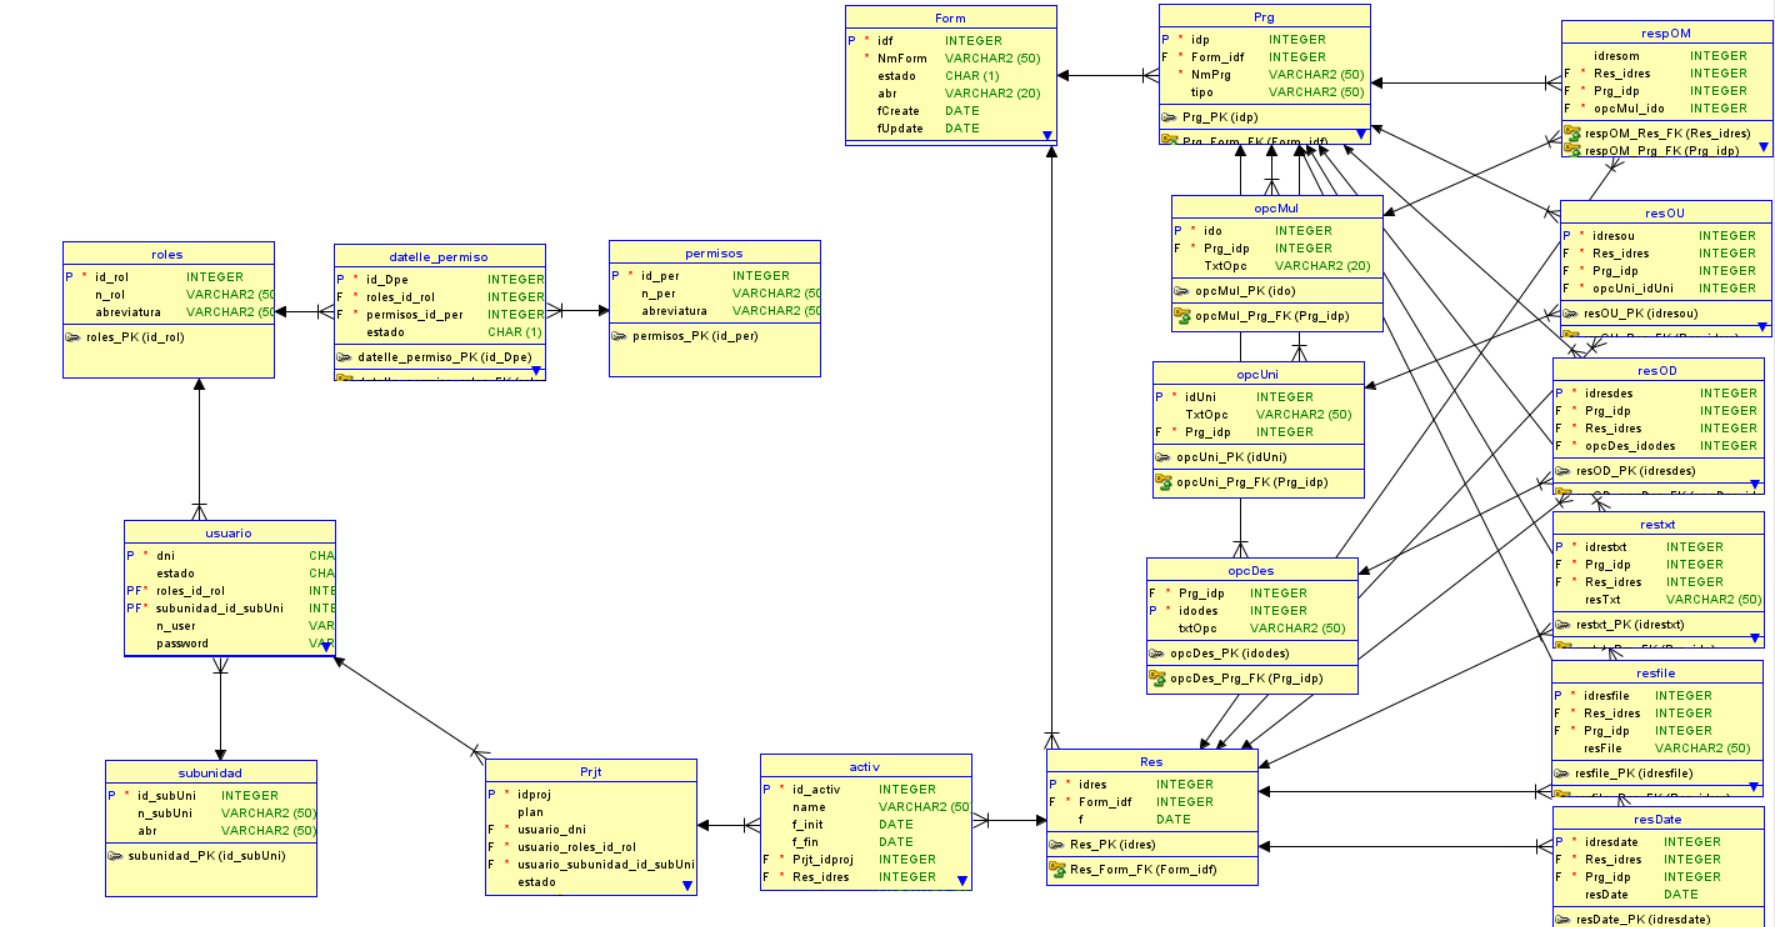
\includegraphics[width=0.8\textwidth]{assets/imagenes/clases.png}
    \caption{Diagrama de Clases del Sistema.}
    \label{fig:clases}
\end{figure}
\FloatBarrier


